\chapter[AprEnDO: o relato de experiência e a analise]{AprEnDO: o relato de experiência e a analise}
\section[Relato de experiência]{Relato de experiência}

\section[Análise]{Análise}

De X alunos na turma, até o momento da última checagem no servidor de dados do \textit{heroku}, contabilizou-se 13 alunos voluntários que enviaram estatísticas, porém não se sabe quantos jogaram. Sabe-se que dos 13 alunos que enviaram, 10 completaram pelo menos uma fase do módulo de classificação e 3 pessoas enviaram as estatísticas sem ter completado nenhuma fase de nenhum módulo. Não se sabe quantas vezes eles tentaram jogar as fases e nem se eles apenas enviaram as estatísticas sem tentar. 

A Figura \ref{est_cla} apresenta o resultado de classificação dos 13 alunos que contribuíram enviando os dados. Onde está escrito falso significa que não foi vencido nenhuma vez a fase (maioria dos casos). E alguns alunos jogaram apenas 1 vez, outros 2 e um aluno jogou 8 vezes.

\begin{figure}[H]
\centering
\caption{Estatísticas colhidas de classificação}
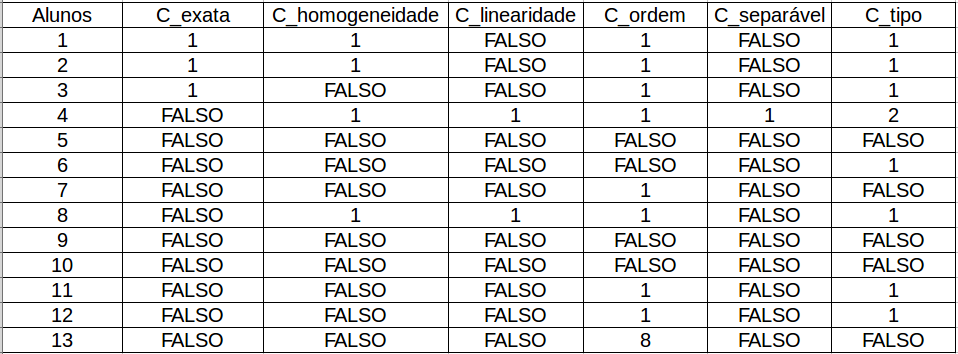
\includegraphics[scale=0.5]{figuras/estatisticas/estatisticas_classificacao.png}
\label{est_cla}
\end{figure}


A Figura \ref{est_res} apresenta o resultado de resolução dos 13 alunos que contribuíram enviando os dados. Onde está escrito falso significa que não foi vencido nenhuma vez a fase (maioria dos casos). E alguns alunos jogaram apenas 1 vez algumas fases, porém a minoria venceu este módulo, percebe-se que sua aceitação não foi muito boa por algum motivo. Apenas 3 alunos jogaram pelo menos 1 vez 1 fase.

\begin{figure}[H]
\centering
\caption{Estatísticas colhidas de resolução}
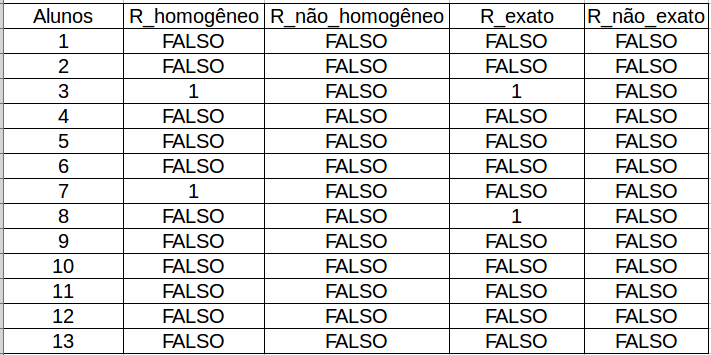
\includegraphics[scale=0.5]{figuras/estatisticas/estatisticas_resolucao.png}
\label{est_res}
\end{figure}

Foi planejado coletar mais dados do servidor, porém por falta de organização do tempo não foi possível coletar todos os dados conforme o planejado. 

Foram planejados desenvolver casos de teste, porém também com o mau planejamento de tempo, a grande dificuldade em desenvolver e executar os testes unitários e de integração automatizados estes acabaram não sendo desenvolvidos.

Abaixo segue uma breve descrição dos testes que foram planejados testar:

\textbf{Testes de servidor no heroku:}
\begin{itemize}
	\item Garantir que cada matrícula seja única. \textbf{OBS:} Apesar do teste não ter sido implementado, existe a checagem na própria função do arquivo para garantir que a matrícula é nula. Foram realizados testes manuais para confirmar que a funcionalidade está funcionando, porém não há testes escritos.  


\item Garantir que os dados recebidos sejam salvos no servidor em arquivo. \textbf{OBS 1:} inicialmente acreditava-se que salvaria os dados no heroku em arquivo, mas percebeu-se que a cada novo envio uma instância era iniciada e os dados antigos não eram persistidos, a ideia foi migrar para a utilização de um banco de dados na nuvem com a ajuda do mLab. \textbf{OBS 2:} Apesar do teste não ter sido implementado, garante-se que os dados recebidos estão sendo salvos no servidor, porém não foram desenvolvidos testes para melhores confirmações e indicações de falhas.  


\textbf{Testes de banco de equações:}
\item Garantir que toda resposta tenha uma pergunta \textbf{OBS:} no próprio desenvolvimento do código da aplicação existe o filtro de selecionar apenas equações com respostas, porém não há testes para a confirmação que o mesmo está funcionando sempre de acordo com o esperado, apesar das muitas validações manuais.  


\textbf{Testes da aplicação react-native:}

	Pacote 1
\item Garantir que carregue todas fases do módulo classificação. \textbf{OBS:} apenas testes manuais e exaustivos foram realizados.  

\item Garantir que carregue todas fases do módulo resolução. \textbf{OBS:} apenas testes manuais e exaustivos foram realizados.  

\item Testar que quantidade de perguntas de classificação é 20. \textbf{OBS:} apenas testes manuais foram realizados.  

\item Testar que quantidade de cartas de resolução sejam 20. \textbf{OBS:} apenas testes manuais foram realizados.  

\item Testar que jogo da memória tenha apenas 10 equações perguntas. \textbf{OBS:} apenas testes manuais foram realizados.  

\item Testar que jogo da memória tenha apenas 10 equações respostas. \textbf{OBS:} apenas testes manuais foram realizados.  

\item Testar que cada pergunta do jogo tenha 1 e apenas uma resposta. \textbf{OBS:} existe apenas o filtro no código da aplicação sem testes escritos.  

\item Testar que apenas duas cartas estejam viradas para cima mostrando seu conteúdo. \textbf{OBS:} apenas testes manuais foram realizados.  

\item Testar em classificação que cada pergunta só tenha uma resposta correta. \textbf{OBS:} apenas testes manuais e exaustivos foram realizados.  

\item Testar em classificação que cada pergunta tenham 4 alternativas diferentes. \textbf{OBS:} apenas testes manuais e exaustivos foram realizados.  


	Pacote 2
\item Garantir que ao enviar estatística a quantidade de vezes jogado zere para o módulo 1 e 2. \textbf{OBS:} apenas testes manuais e exaustivos foram realizados.  

\item Garantir que ao enviar estatística o tempo  total de cada fase zere para o módulo 1 e 2. \textbf{OBS:} Não foi coletado o tempo jogado de cada fase.  

\item Garantir que ao enviar estatísticas ao servidor a informação a respeito das fases completas nos módulos permaneça a mesma e zere apenas quantas vezes foi vencido. \textbf{OBS:} apenas testes manuais e exaustivos foram realizados.  
\end{itemize}

Não foi medido o tempo total gasto com o desenvolvimento dos códigos e nem o custo. O único custo que o projeto teve foi a licença da google play para poder publicar o jogo. O valor da licença foi de 25 dólares, aproximadamente 110 reais. 
